%%%%
% -- Data Science
% --     FOBOS Keck White Paper 2019
%%%%

\subsection{FOBOS as an ideal spectroscopic training instrument}
\label{sec:datascience}

FOBOS will provide observations that directly lead to invaluable
science. However, FOBOS will also allow teams of Keck scientists to
quickly build spectoscopic samples purposely designed to be used in
training machine-learning algorithms. These data will allow us to
statistically infer physical properties from upcoming large-scale
broad-band imaging surveys (e.g., LSST, WFIRST, Euclid) that are only
directly accessible via spectroscopy and complement more shallow
spectroscopic surveys made with FOBOS or surveys using smaller
aperture facilities (e.g., APOGEE, DESI). Keying off one of NSF's ten
Big Ideas, we highlight a few ways that FOBOS can be used to "harness
the data revolution."

\comment{these sections need to be shortened}

\begin{figure}[h!]
%
\vskip -0.1in
%
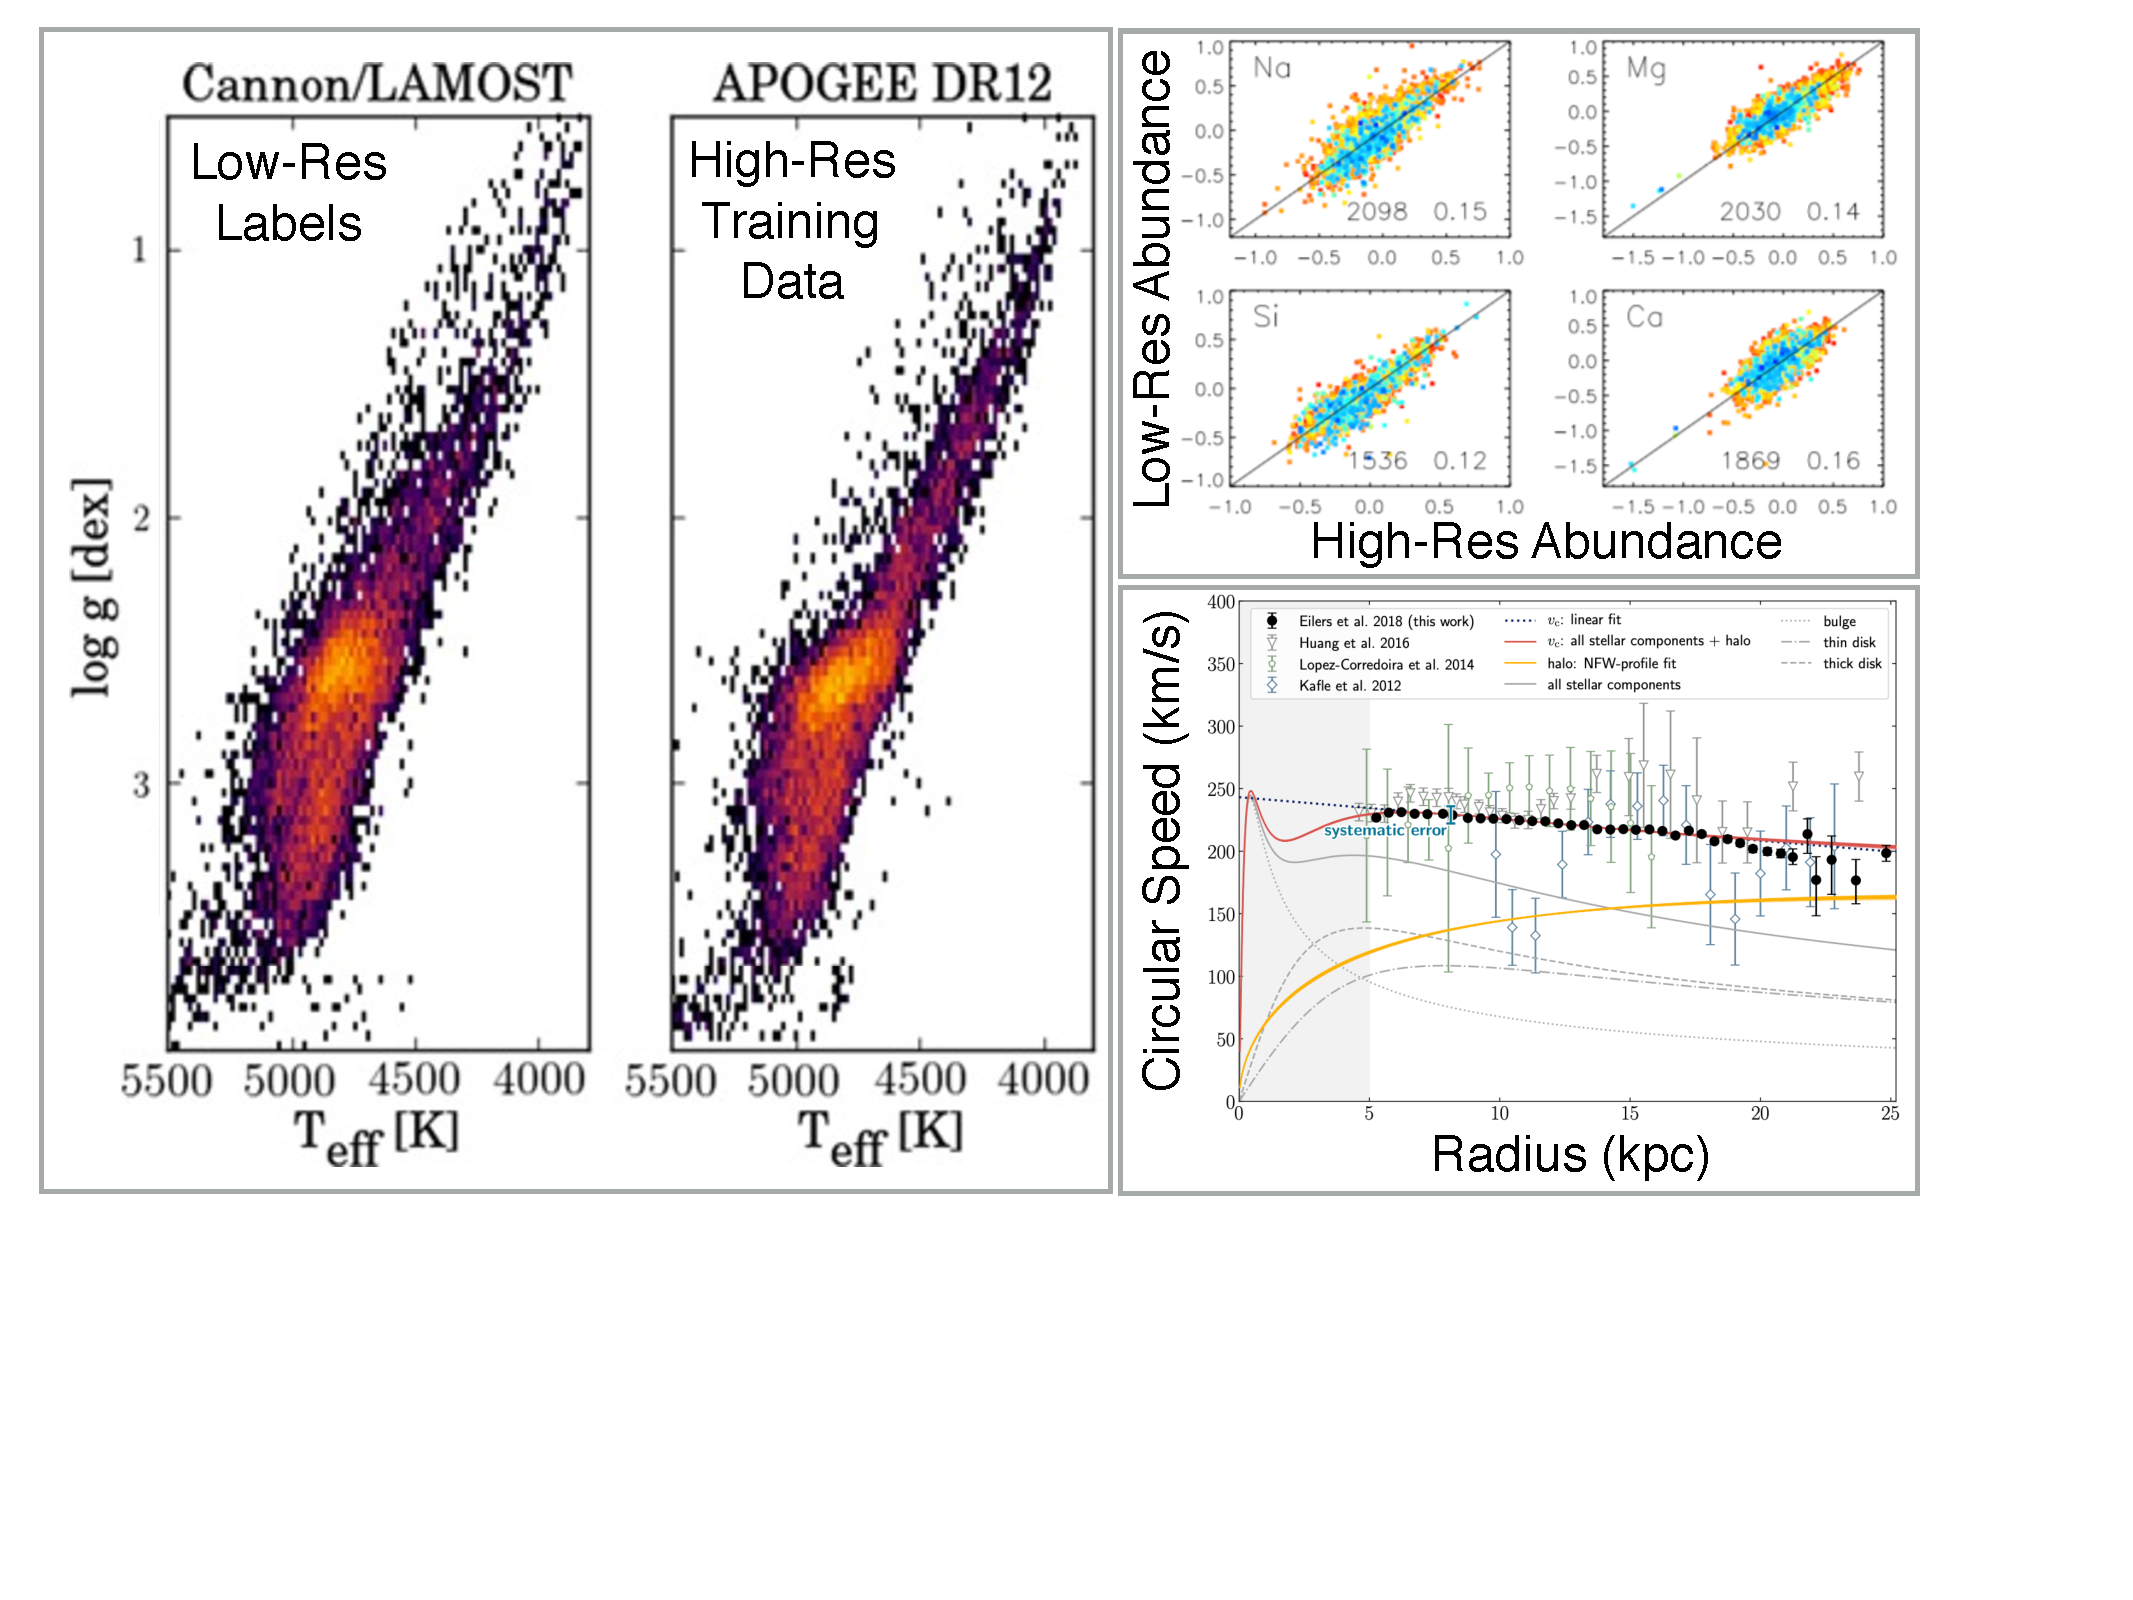
\includegraphics[width=\textwidth]{figs/LGplots.pdf}
%
\caption{{\it Left}: Validation of {\it The Cannon} measurements of
stellar effective temperature, $T_{\rm eff}$, and surface gravity, $\log
g$, using low-resolution LAMOST spectra (left) compared to
high-resolution APOGEE measurements
\citep[right;][]{2017ApJ...836....5H}. {\it Top-right}: Recovery of
elemental abundances from low-resolution LAMOST spectra compared to
high-resolution measurements from GALAH (Xiang et al., in prep).  {\it
Bottom-right}: The circular-speed curve of the Milky Way determined
using a data-driven model that combines stellar parameters determined
from APOGEE spectra with photometry from WISE, 2MASS, and Gaia, yielding
the most precise measurements to date \citep{2019ApJ...871..120E}.}
%
\label{fig:Cannon}
%
\end{figure}

\subsubsection{The chemical evolution of Milky Way stellar populations}
Radial velocity studies of stars in the MW halo or the M31 disk require
observations of up to 10 hours on large telescopes
\citep[e.g.,][]{2018arXiv180904082C}.  This again motivates
machine-learning algorithms to extract physical quantities from both
multi-band imaging and lower quality spectra (low resolution and S/N)
using relatively small, yet high-S/N, training sets.  For example,
\citet{2015ApJ...808...16N} have developed {\it The Cannon}, a
supervised learning approach that uses spectra with known stellar
parameters to label spectra where those parameters are unknown
(Fig.~\ref{fig:Cannon}).  Additionally, \citet{2018arXiv180401530T} have
developed {\it The Payne} which can infer 16 stellar-abundance labels
from low-resolution spectra using a neural network and theoretical
stellar spectra.  Finally, \citet{2018arXiv180803278T} have combined
Kepler-based astroseismology measurements with APOGEE spectra to
determine stellar age to $\sim$25\% precision using a neural network.
Our proposed effort builds on new lines of inquiry based on these
successes.

A nested network of stellar parameter training samples for resolved
Milky Way and Local Group studies via extracting maximum information
from photometry, in this case stellar parameters. Our goal is to
reach magnitudes significantly fainter than the detection limit of
current and upcoming spectroscopic surveys of the Milky Way including
Gaia, APOGEE,\footnote{APOGEE, the Apache Point Observatory Galaxy
Evolution Experiment has observed in both SDSS-III and SDSS-IV.} the
SDSS-V Milky Way Mapper, planned programs with 4MOST\footnote{4MOST:
4-meter Multi-object Spectroscopic Telescope.} and the Dark Energy
Spectroscopic Instrument (DESI) Milky Way Survey, among others.
Inferring stellar parameters beyond V$\sim$18 will open up studies of
the Milk Way's outer halo, the halo of M31, and stellar populations
in local dwarf galaxies.

The immediate challenge is to design an optimized, nested set of
training samples that connect data from the surveys above. This
nested set will span high-S/N to low-S/N and high spectral resolution
to low spectral resolution for sufficiently large, overlapping
stellar samples. Subsets will have astroseismology from
TESS\footnote{TESS is NASA's Transiting Exoplanet Survey Satellite.}
and PLATO.\footnote{PLATO is ESA's PLAnetary Transits and
Oscillations mission.} Using simulated spectra with known input
parameters, we will test methods for ``label transfer'' from
information-rich spectra to information-poor spectra as we work down
to fainter magnitudes, landing eventually at multi-band photometry
alone. Within this nested set, low-resolution FOBOS data will fill in
gaps at both high-S/N, where we will be training FOBOS data on higher
resolution spectroscopy, as well as lower-S/N where we will be
training photometry on FOBOS spectroscopy. The success of this
multi-layered label transfer depends not only on the size of the
training sets we can access or observe, but on how representative
they are. Label transfer to WFIRST imaging of the M31 halo, or Local
Group dwarfs in either hemisphere, is a particular concern. We will
test it by evaluating label recovery on simulated stellar spectra
with cosmologically informed formation histories for M31 and dwarf
galaxies, suitably differentiated from the Milky Way stars that
anchor the training network.

\comment{Raja, Ting: Help with shortening/refocusing the above}

\subsubsection{The $z$$\sim$2 Galaxy Population}

For decades, we have used the spectral information encoded in
broad-band photometry to infer properties of galaxies beyond their
color and brightness. The most common application is to estimate the
galaxy redshift from its broad-band colors, i.e. photometric
redshifts (photo-$z$s). However, as demonstrated in Figure
\ref{fig:SOM}, the range of observed spectral types is
well-constrained by broad-band imaging, suggesting a far greater
potential for imaging data to reveal physical properties with
sufficient training of deep-learning algorithms.  These properties go beyond what conventional modeling of spectral energy
distributions (SEDs) would suggest. The challenge here is to identify
the extent to which machine learning can deliver SDSS-like
information --- e.g., star-formation histories, stellar-population
properties, dust content, inflow/outflow properties, and stellar
masses --- and determine design parameters for future training sets
that will enable such inferences for millions of imaged galaxies at
$z$$\sim$2.

Self-Organizing Maps (SOM, Figure \ref{fig:SOM}) provide a
state-of-the-art representation of a high-dimensional input space in
projected 2D grid cells, allowing us to benchmark sampling of the
photometric color space under various training set designs. We will
also use Bayesian Optimization techniques to evaluate the success of
simulated training sets against the fidelity of full cosmological
analyses that employ them. This will enable extremely rapid
exploration of the optimal design space.

\comment{Master, Mandelbaum, Rau, Schafer}

\begin{figure}[h!]
\vskip -0.1in
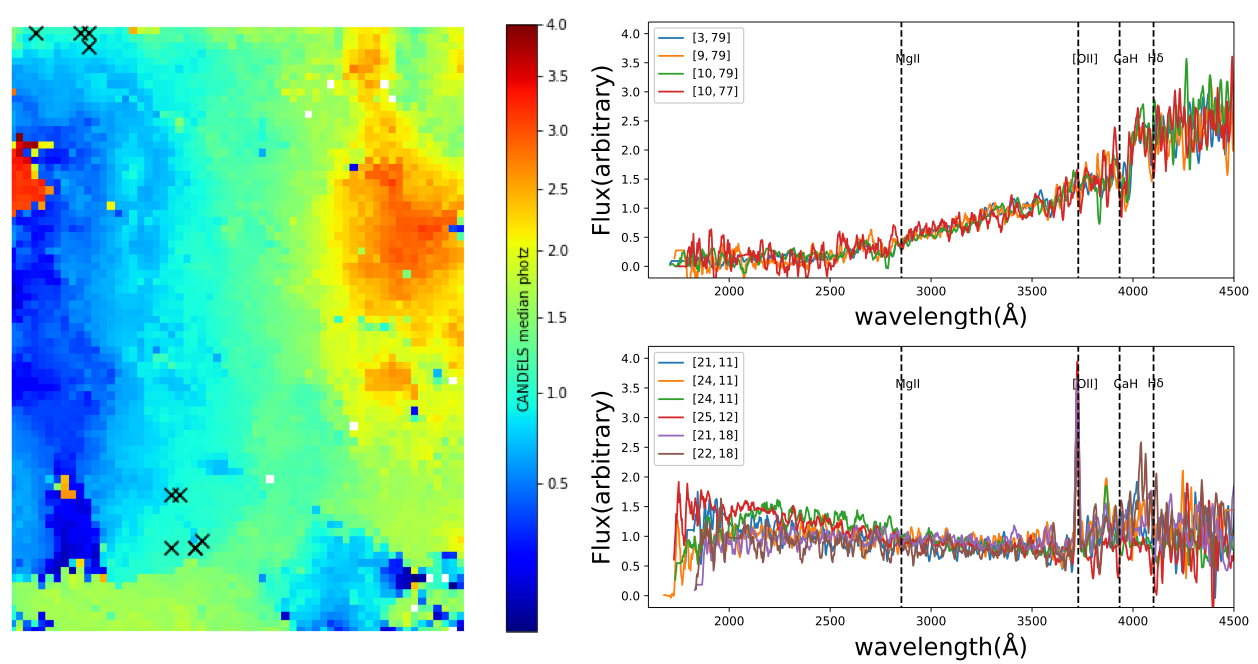
\includegraphics[width=\textwidth]{figs/Hemmati18_Fig8_VVDS_spec.png}
\caption{\small {\it Left}: A Self-Organizing Map
\citep[SOM;][]{1990Natur.346...24K} from \citet{hemmati18} encoding
the relation between colors in an LSST+WFIRST-like color space and
redshift, $z$. Position in the SOM is associated with a position in
the multi-dimensional broad-band color space of galaxies. Galaxies
observed in this space are assigned $z$ values based on the median
photo-$z$ of galaxies from the CANDELS survey \citep[color
bar;][]{2011ApJS..197...35G}. Such SOMs can be used to optimally
define spectroscopic training samples for use with imaging surveys.
{\it Right}: Galaxy spectra from VVDS \citep{2005A&A...439..845L};
black crosses near the top and bottom of the SOM are plotted in the
top and bottom panels, respectively. Note the similarity of the
high-resolution spectra associated within the SOM, suggesting that a
systematic spectroscopic exploration of the LSST color space would
have far-reaching benefits to the science return of the mission
beyond the photo-$z$ application.}
\label{fig:SOM}
\end{figure}

% The complete photo-$z$ training survey described in \citet{newman15}
% would require 15 independent pointings, each spanning 0.1 deg$^2$ with
% a target density of 6 arcmin$^{-2}$ (8 arcmin$^{-2}$ when including $z
% > 1.5$ galaxies accessible in the UV with Keck-FOBOS), perfectly
% matched to the Keck-FOBOS field-of-view and target density.  With a
% conservative exposure time of 100 hours to reach 75\% redshift
% completeness for 40,000 galaxies with $i_{\rm AB} < 25.3$, the Neman
% survey would require 400 nights.  Challenge \ref{photoz} would reduce
% the required survey duration by a factor of at least four.  Meanwhile
% the extreme depths and flux-limited selection are likely also
% requirements for training sets associated with Challenges \ref{phot},
% \ref{uv}.

% A wider and shallower survey component is envisioned for Challenges
% \ref{lowsnr} and \ref{gaia}.  With 10-minute integrations, a 52
% deg$^2$ Keck-FOBOS sample of environmental diagnostics for 1 million
% galaxies could be carried out in less than 20 nights.  This program
% would sample at $z \sim 1.5$ the same cosmic volume as SDSS.  A
% program of a similar scale would provide training set data for
% inference of stellar parameters in the Milky Way.  These shallow
% programs would be integrated with the deeper components described
% above into a single survey plan.